\documentclass[a4paper,12pt]{article}

\title{Exercise 2: Obstacle Avoidance}
\author{Gruppe 6:  \\ Niels \\ Troels \\ Mark \\ Kristian}

\usepackage[T1]{fontenc}
\usepackage[utf8]{inputenc}
\usepackage{lmodern}
\usepackage[british]{babel}
\usepackage{microtype}

\usepackage{amsmath}
%\usepackage{libertine}

\usepackage{graphicx}

\usepackage[hidelinks]{hyperref}

\setlength{\parskip}{1ex}
\setlength{\parindent}{0pt}
\setlength{\parfillskip}{30pt plus 1 fil}

\begin{document}

\maketitle

\section{Measurements}

We started by measuring the robot's front IR sensor on seven distances: 0 cm, 10
cm, 20 cm, 30 cm, 40 cm, 50 cm, and 60 cm.  We positioned the robot in front of
pieces of paper in a lit room and had it make 20 IR measurements at each
distance.  The distance was from the robot's bumper to the piece of paper.


\section{Driving}

\subsection{Issue: Pull mode vs. push mode}

We had a problem with wrong IR readings on the Scorpion robots \emph{and} in the
Stage simulator.  When not constantly calling the \texttt{Read()} function, the
\texttt{libplayer} API sometimes gave us old readings instead of current ones.
After doing some research, we found out that the issue was because of how the
default data mode was used by
\texttt{libplayer}\footnote{\url{http://playerstage.sourceforge.net/doc/Player-cvs/player/group__libplayerc__datamodes.html}}.
By default it uses PULL mode.  This mode sends messages to the client when asked
to, but if the client does not read often enough, buffer overflows in the server
queue can occur.  To get rid of this problem, and not have to call
\texttt{Read()} all the time, we have set a \texttt{libplayer} replace rule:

\begin{verbatim}
robot.SetReplaceRule(true, PLAYER_MSGTYPE_DATA, -1, -1);
\end{verbatim}

This rule tells \texttt{libplayer} to ignore the buffer queue and just replace
every old measurement with every new measurement, thus ensuring that
\texttt{Read()} gets us the newest measurement.

\subsection{Abortmission}

Our first test program Abortmission worked by driving straight forward at 20 cm/sec forever. While checking every 20 ms, if the front ir sensor detected anything within 50 cm. If so we would stop and turn 180 degrees/sec left or right for 1 second. We determined the turning direction by comparing the distance readings of the left and right ir sensor relative to the center ir sensor, shown as red and blue in figure 1. We always turn towards the longest sensor reading of the two. If they were equal we would turn right.
\newline
\newline
This solution just barely worked, since it only used the front sensor and arbitrarily just turned 1 second in the chosen direction.

\begin{figure}[!h]
\centering
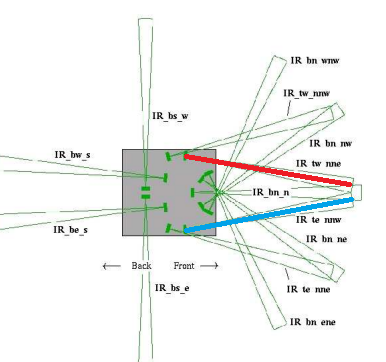
\includegraphics[scale=0.7]{robot2.png}
\caption{Robot sensors}
\end{figure}
\subsection{Sensor-validate}

We initially implemented Sensor-validate to only believe a sensor if it read out a valid distance within our threshold 10 times in a row, otherwise its counter would be reset. This was to ignore invalid readings but ended up making us never believe any sensors. Therefore we changed it to just see any sensor reading, within our threshold, as a potential collision.
\newline
\newline
Sensor-validate works by having the robot drive straight forward at 20 cm/sec forever. If any of the 9 front mounted sensors detect anything within 50 cm we stop and turn left at 30 degrees/sec until no sensors detect anything. 
\newline
\newline
This solution worked well as the robot would stop, with a good safety distance counting for deceleration, and turning until nothing was in its way, before continuing. This solution was not perfect as the ir sensors could not reliably detect table legs, round objects or reflective surfaces as it wouldn't get accurate sensor readings.

\newpage
\section{Sensor Calibration}

We implemented a program called ir-measurements to make a ir calibration function. The program asks the user whether he's ready to measure at a specified distance and then makes 20 measurements using the front ir-sensor (IR\_bn\_n). When the measurements are done the program asks you if you are ready to make new measurements for the new specified distance. Once the distances 0, 10, 20, 30, and 40 centimeters are measured, the program then writes it to a file.

This program was run with both a green and a pink surface to check if there was any difference on the ir readings dependent on the color.

The data in the output file was then processed in a Python Script. First we made a Scatter-plot of both the output files and made a linear regression of them. The green dots and line refers to the green data sample and vice versa.   

\begin{figure}[!h]
\hspace{-6cm}
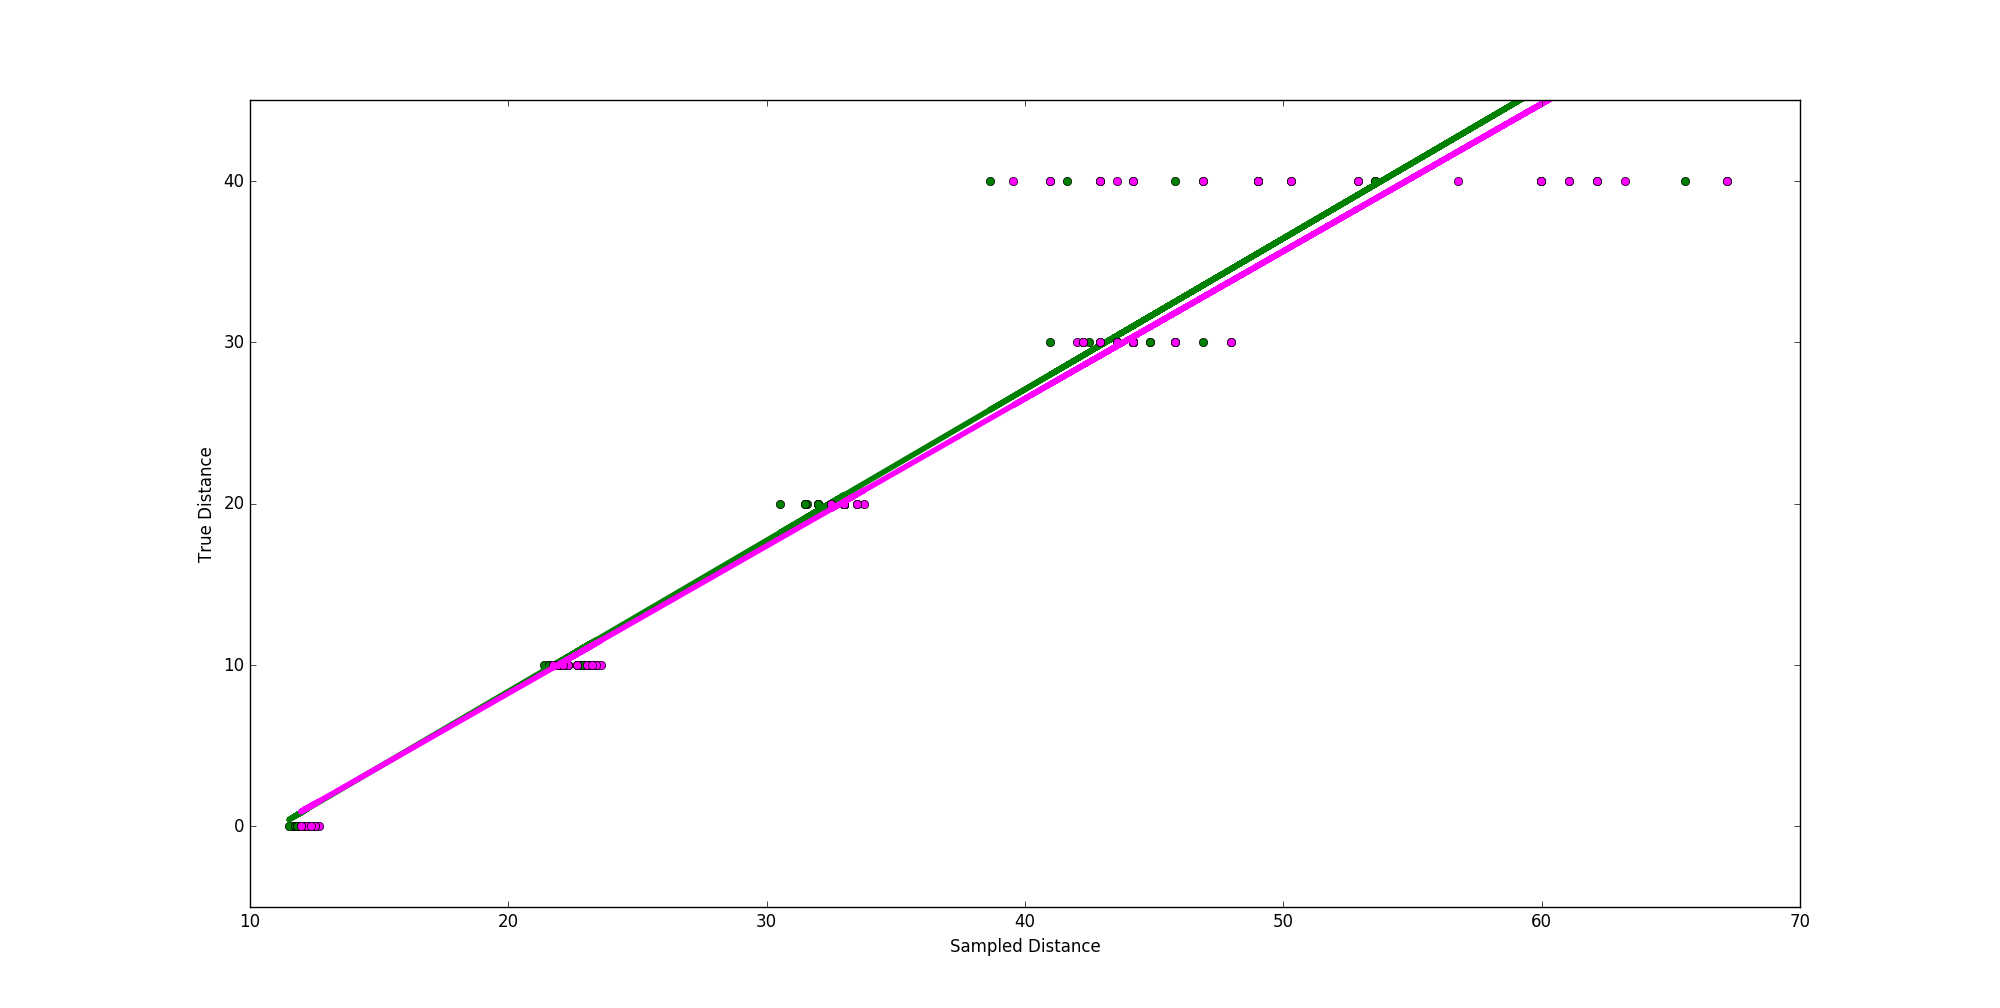
\includegraphics[scale=0.5]{reg_mix}
\caption{Regression on sample data from both surfaces}
\label{fig:mixed_reg}
\end{figure}

We found the following fits for $y = a\cdot x + b$:\\
Green: $0.935690446778\cdot x-10.3488330212$\\
Pink: $0.913109248489\cdot x-10.0141712782$

We noticed that the average, of the data measured at the distance of 0, was 11.91. This observation suggests, that we do believe that our b-value should be nearer $-11.91$. 
The data also suggests that the ir-measurements are more precise on a green surface.
\newpage

This observation lead us to the next plots where we calculated the Standard Deviation for each of the two samples. We then plotted the samples separately with error boxes for each measured distance.   
This plot also clearly illustrates that the further away the measurement is, the more imprecise the readings are.  

\begin{figure}[!h] 
\hspace{-6cm}
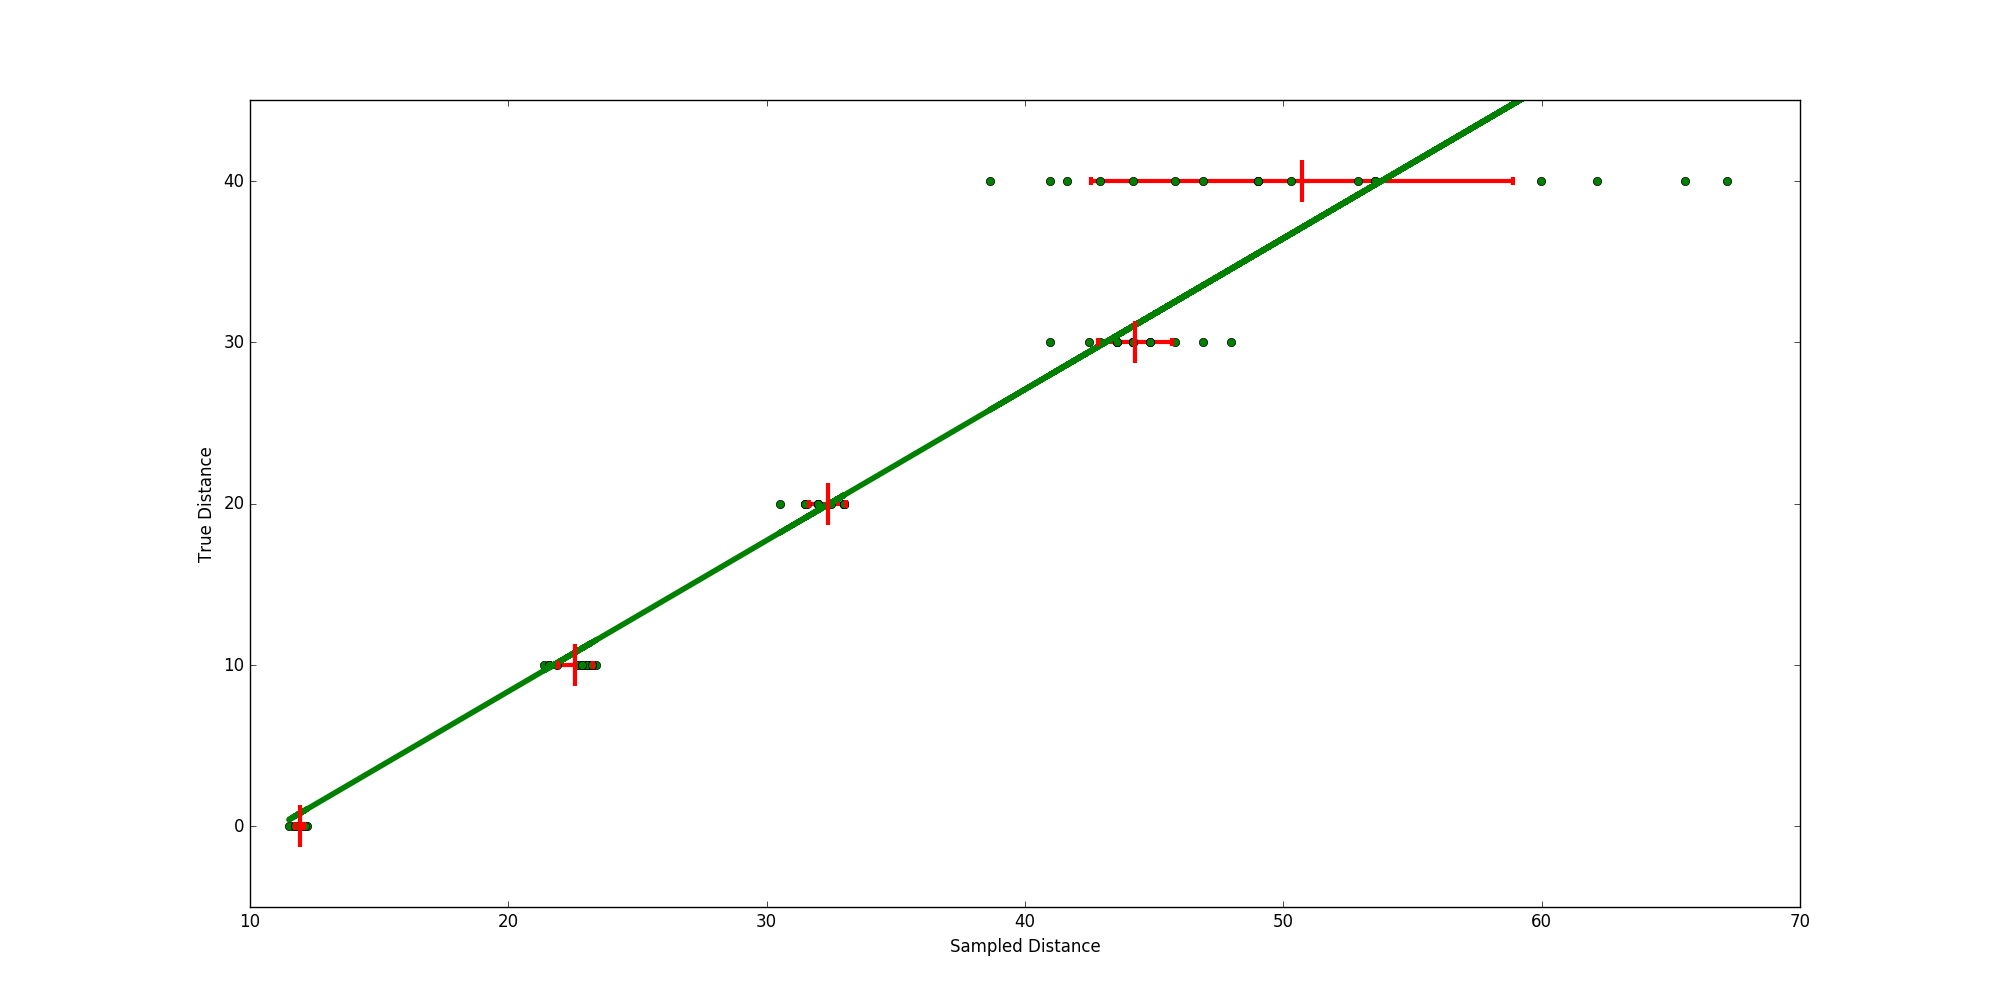
\includegraphics[scale=0.5]{reg_green}
\caption{Regression on sample data from green surface}
\label{fig:green_reg}
\end{figure}
\begin{figure}[!h]
\hspace{-6cm}
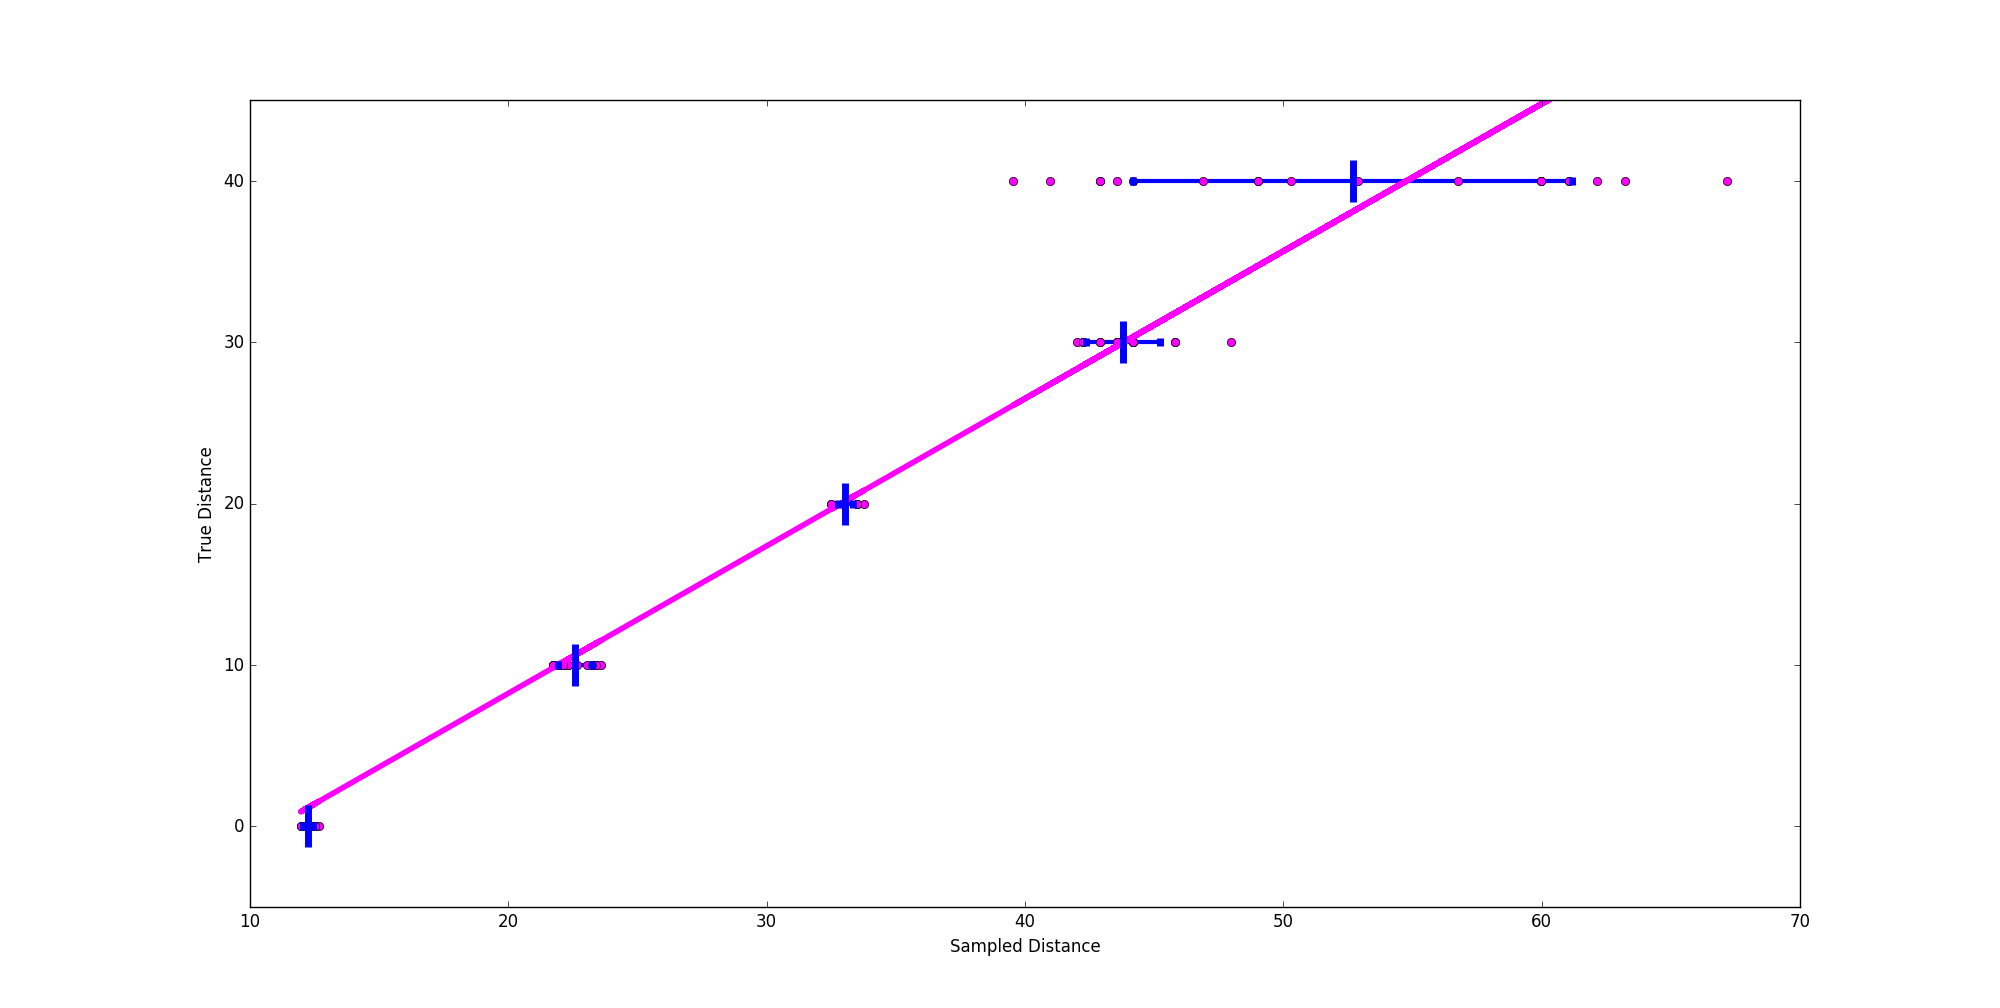
\includegraphics[scale=0.5]{reg_pink}
\caption{Regression on sample data from pink surface}
\label{fig:pink_reg}
\end{figure}

\end{document}
